\chapter{p-p Interactions and their Simulation}
\label{chap:event:MC}


\gls{pp} interactions at the \gls{lhc} are complicated processes that span very different energy scales. 
To interpret the \gls{lhc} data it is important to both 
develop a good understanding of the physics taking place during a \gls{pp} collision and also be able to simulate 
it, to allow a comparison of the observed data with data simulated based on a specific theory, first of all the \gls{sm}.
Section \ref{sec:ppint} focuses on the description of our understanding of a \gls{pp} collision, while Section \ref{sec:eventsimul} 
discusses the event-simulation process and the main \gls{mc} generators used in the \gls{atlas} Collaboration. 



\section{p-p Interactions}
\label{sec:ppint}

In hard-scattering processes, where the momentum transfer is much higher than the proton mass \cite{Butterworth:2012fj}, 
a \gls{pp} collision is easier to understand in terms of interactions between the constituents of the protons, quarks and gluons, 
collectively referred to as partons. A schematic view of \gls{pp} event is shown in Fig. \ref{fig:sim:pp2}. In this case, the interaction of a quark and a gluon leads to a final state with a Z boson and jets. 


\begin{figure}[h]
\begin{center}
%  \subfigure[]{
%    \label{fig:Comb_syst:pt}
    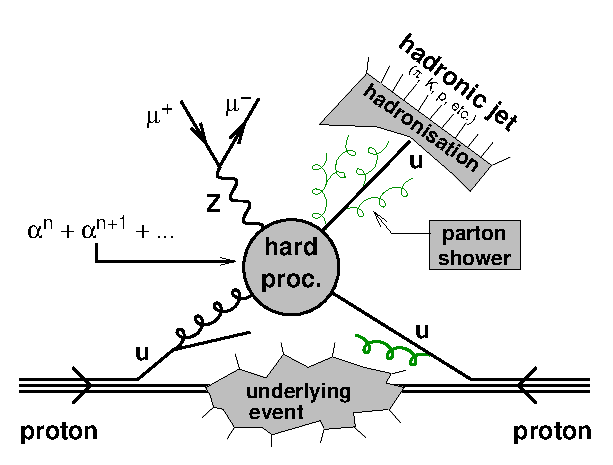
\includegraphics[width=0.58\textwidth]{figures/simul/ppcoll2}
%  }
\end{center}
 \caption{Schematic representation of a \gls{pp}, involving a quark-gluon scattering that leads to a final state consisting of a Z boson and a hard jet. Figure from Ref. \cite{Butterworth:2012fj}.}
  \label{fig:sim:pp2}
\end{figure}


The hard scattering between the partons inside the proton is in a kinematic regime where the \gls{qcd} coupling constant, $\alpha_s$, 
is small and therefore the partonic cross sections can be computed in perturbation theory. Instead, our understanding of the 
low-energy hadronization process, where stable hadrons are formed, is based on phenomenological models.

The generic production cross section for a final state $X$ can be expressed in terms of the partonic cross section $\hat\sigma$ as:

\begin{equation}
  \label{eq:general-cross-section}
  \sigma(pp\rightarrow X) = \sum_{i,j} \int dx_1 dx_2\, 
     f_{i,p}(x_1,\mu_F^2)\, f_{j,p}(x_2,\mu_F^2)\, 
     \hat\sigma_{ij\rightarrow X}(x_1 x_2 s, \mu_R^2, \mu_F^2) \; .
\end{equation}

The $i$ and $j$ indexes run on all the possible partons.  

The partonic center of mass energy \cmpart is lower than the total center of mass energy, as it is the product of the center of mass energy times
the fraction of the proton momentum that is carried by each parton. 

\subsection{Hard Scattering}

\cite{doi:10.1146}

\begin{figure}[h]
\begin{center}
%  \subfigure[]{
%    \label{fig:Comb_syst:pt}
%    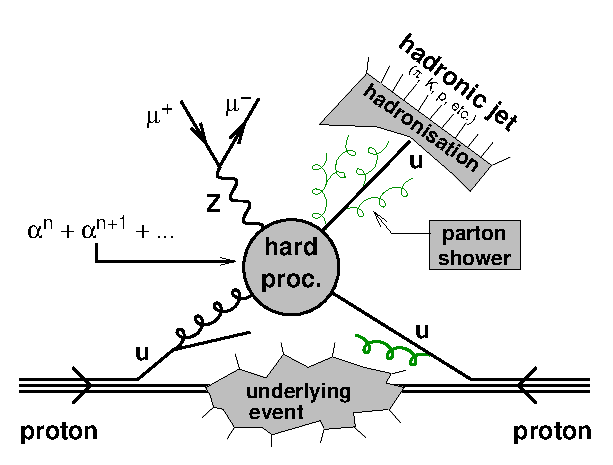
\includegraphics[width=0.48\textwidth]{figures/simul/ppcoll2}
%  }
%    \subfigure[]{
%    \label{fig:Comb_syst:pt}
    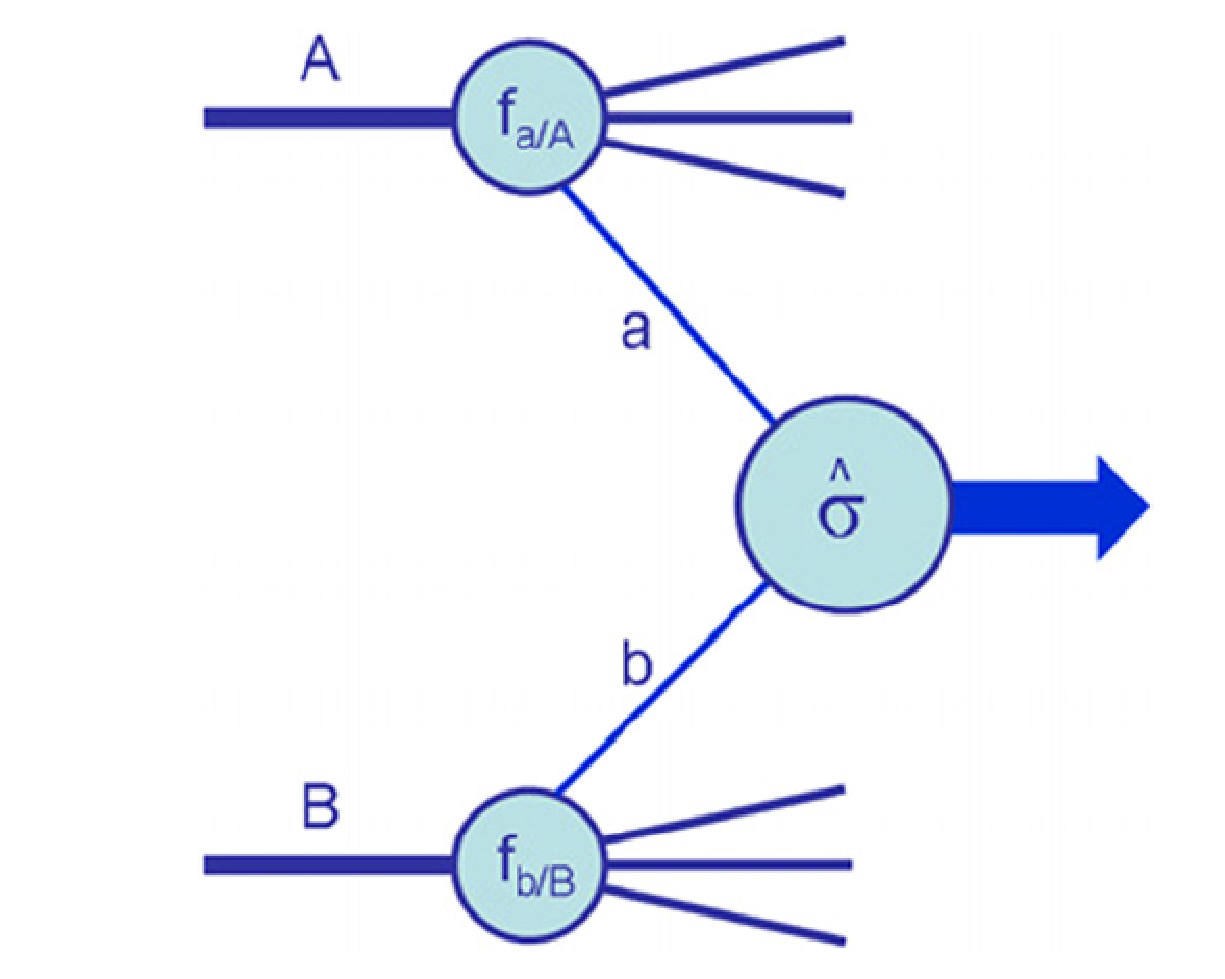
\includegraphics[width=0.48\textwidth]{figures/simul/ppcoll}
%  }
\end{center}
 \caption{Diagrammatic structure of a generic hard-scattering process. Figure from Ref. \cite{Campbell:2006wx}.}
  \label{fig:sim:pp}
\end{figure}

\subsection{Parton Density Functions}

\begin{figure}[h]
\begin{center}
    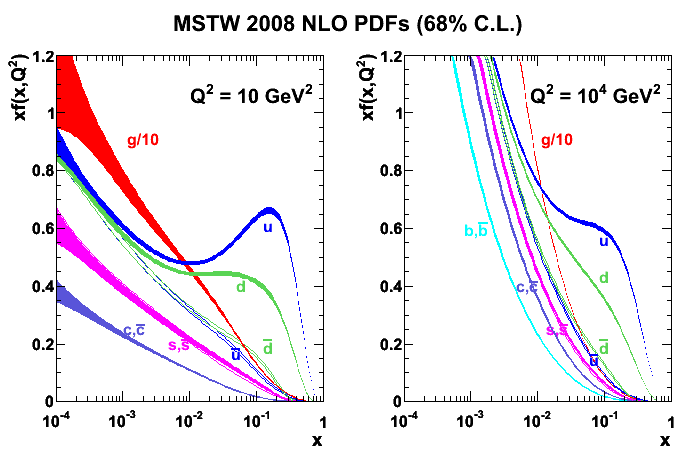
\includegraphics[width=0.8\textwidth]{figures/simul/pdf}
\end{center}
 \caption{MSTW 2008 NLO PDFs at Q$^2$ = 10 GeV$^2$ and Q$^2$ = 104 GeV$^2$. Figure from Ref. \cite{Martin:2009iq}.}
  \label{fig:sim:pp}
\end{figure}


\section{Event Simulation}
\label{sec:eventsimul}

\subsection{Matrix Element}

\subsection{Parton Shower}

\subsection{Matching}

\subsection{Hadronization}

\section{MC Generators}

\section{Detector Simulation}

\section{Data-driven Corrections}
